\documentclass[12pt]{article}
\usepackage[paper=a4paper,left=30mm,right=30mm,top=35mm,bottom =35mm]{geometry}
\usepackage[utf8]{inputenc}
\usepackage[T1]{fontenc}
\usepackage{stmaryrd}
\usepackage{setspace}
\usepackage{mathrsfs}
\usepackage[ngerman]{babel}
\usepackage{amssymb}
\usepackage{amsmath}
\usepackage{fancyhdr}
\usepackage[dvips,unicode,colorlinks,linkcolor=black]{hyperref} 
\usepackage{graphicx}
\usepackage{float}

\pagestyle{fancy}
\lfoot{}
\rfoot{Paul Kremser, Tobias Grussenmeyer}
\cfoot{\thepage}
\fancyhead[L]{FPI Versuch: Halbleiter}
\renewcommand{\headrulewidth}{0.6pt}
\renewcommand{\footrulewidth}{0.6pt}
\setlength{\headheight}{16pt}
\setlength{\parindent}{0pt}
% Für die Wahl der Schriftart
\newcommand{\changefont}[3]{
\fontfamily{#1} \fontseries{#2} \fontshape{#3} \selectfont}

\begin{document}
% keine Hurenkinder und Schusterjungen
\clubpenalty = 10000
\widowpenalty = 10000 
\displaywidowpenalty = 10000

\onehalfspacing
% Schriftart
\changefont{ptm}{m}{n} 

\begin{titlepage}
\author{Paul Kremser, Tobias Grussenmeyer}
\title{Versuch: Halbleiter}
\date{Versuchsdurchführung: 5. November 2009} 
\maketitle
\thispagestyle{empty}
\end{titlepage}


\tableofcontents
\thispagestyle{empty}
\newpage
\pagenumbering{arabic}
\section{Überblick}

\section{Aufgabestellung}
\subsection{Vermessung der Bandlücke}
\begin{itemize}
 \item Optimieren Sie den Strahlengang für das Licht des Spektrometers. Beachten
Sie dabei, dass das optische Gitter und der verwendete Filter zu der
ausgewählten Halbleiterprobe passen.
 \item Verwenden Sie die Software “LoggerPro”, um bei jeder der beiden zu
Verfügung stehenden Halbleiterproben (Silizium, Germanium ) ein
Absorptionsspektrum und ein Transmissionsspektrum aufzunehmen.
 \item Führen Sie für beide Spektren eine Untergrundmessung durch.
 \item Vermessen Sie die Strahlungsleistung der Lampe + Filter.
 \item Überlegen Sie sich eine Möglichkeit, um Fehlerbalken auf die Messungen der
Spektren zu errechnen.
 \item Bestimmen Sie den Wert der Bandlückenenergie von Germanium und
Silizium aus dem Transmissionsspektrum.
 \item Bestimmen Sie den Wert der Bandlückenenergie von Germanium und
Silizium aus dem Absorptionsspektrum.
\end{itemize}

\subsection{Haynes- und Shockley-Experiment}
\begin{itemize}
 \item Beobachten Sie die zeitliche und räumliche Entwicklung einer
Ladungsträgerwolke, die von einem Laserpuls in einer Germaniumprobe
erzeugt wurde.
 \item Vermessen Sie diese Entwicklung: Die Ladungsträgerwolke wird von einer
Treiberspannung von dem Auftreffpunkt des Lasers zu der Prüfnadel des
Oszilloskops bewegt. Variieren Sie in zwei Messreihen zum einen den
Abstand
Nadel-Laserpunkt und zum anderen den Wert der Treiberspannung.
 \item Berechnen Sie aus der zeitlichen Entwicklung des Schwerpunkts der
Ladungsträgerwolke die Beweglichkeit $\mu_e$ freier Elektronen in $p$-Germanium.
 \item Berechnen Sie aus der zeitlichen Entwicklung der Signalstärke der
Ladungsträgerwolke die mittlere Lebensdauer $\tau_e$ freier Elektronen in
$p$-Germanium.
 \item Berechnen Sie aus der zeitlichen Entwicklung der Ladungsträgerwolke
(Standardabweichung einer Gaußkurve) die Diffusionskonstante $D_e$ für freie
Elektronen in $p$-Germanium.
\end{itemize}

\subsection{Halbleiterdetektor}
\begin{itemize}
 \item Machen Sie sich mit dem Aufbau des Detektors und der dazugehörigen
Elektronik vertraut
 \item Vermessen Sie das Spektrum von $^{57}Co$ und $^{241}Am$ mit einer Silizium-Diode
 \item Vermessen Sie das Spektrum von $^{57}Co$ und $^{241}Am$ mit einem CdTe-Kristall
(Cadmiumtellurid und Gold: Ohmscher Kontakt)
 \item Berechnen Sie aus dem Verhältnis der Peakhöhen das Verhältnis der
Absorptionswahrscheinlichkeiten von Silizium und $CdTe$
 \item Berechnen Sie aus Lage und Breite der Peaks die relative
Energieauflösung
\end{itemize}

\section{Theoretische Grundlagen}
\subsection{Vermessung der Bandlücke}
Für die Vermessung sollen in einem Halbleiter durch photonische Anregung elektronen vom Valenz- ins Leitungband gehoben werden. Durch Variation der Photonenenergie soll mittels Messung der Apsorption im Halbleiter und Transmission durch diesen die Breite der Bandlücke festgestellt werden. Hierbei soll angenommen werden dass die Breite der Bandlücke ungefähr der Energie entspricht welche irgentwo zwischen Einsetzen der Absorprion und aussetzen der Transmission liegt.

\subsubsection{Bändermodell}
Betrachtet man ein einzelnes Atom, liegen die Energieniveaus der Elektronen des Atoms in diskreter Form vor. Dies gilt 
auch für weit voneinander entfernte Atome. 
Nähert man zwei Atome einander an, so tritt ein Effekt auf der dem Verhalten gekoppelter Pendeln ähnelt, die Anzahl der möglichen Schwingungsfrequenzen erhöht sich. Bei Atomen im Gitter spalten sich die Elektronenniveaus
der Elektronen der beiden Atome auf (Pauliprinzip, keine Doppelbesetztung der Energien). Die Energieniveaus 
verschieben sich jeweils leicht nach oben und unten. Betrachtet man nun einen Kristall, bei dem eine Vielzahl 
von Atomen miteinander wechselwirken, steigt die Anzahl der erlaubten Energiezustände entsprechend, sie 
verschmieren zu \textbf{Energiebändern}.\\

Dies ist eine vereinfachte, anschaulichere Erläuterung. Physikalisch exakt entstehen die Bänder durch Superponierung der
atomaren Orbitale, wenn diese hinreichend überlappen, oder anders gesagt: aus der Lösung der Schrödingergleichung für
ein einzelnes Elektron im Feld der Ionenrümpfe.\\

Die Breite der Energiebänder ist für die unterschiedlichen Energieniveaus nicht gleich. Der Grund dafür ist
die unterschiedlich starke Bindung der Elektronen an ihr Atom. Elektronen auf niedrigen Energieniveaus sind stärker
gebunden und wechselwirken weniger mit Nachbaratomen. Dies führt zu schmalen Bändern. Die Valenzelektronen im Valenzband
(bei Metallen dem Leitungsband) sind leichter gebunden und können daher die Potentialberge zwischen den Atomen
einfacher überwinden. Sie wechselwirken stark mit denen der Nachbaratome und lassen sich in einem Kristall nicht mehr 
einem einzelnen Atom zuordnen, diese Bänder werden dabei breiter, siehe Abbildung.

\begin{figure}[H]
\centering
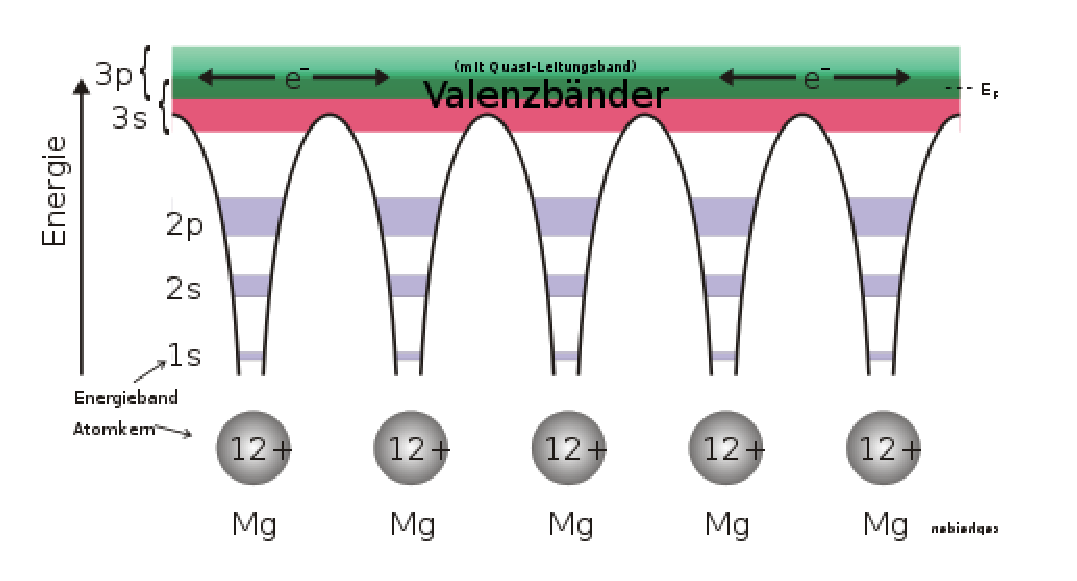
\includegraphics[width=0.9\linewidth]{pictures/baendermodell.eps}
\caption{Bändermodell - Potentialtöpfe}
\end{figure}

\textbf{Einteilung anhand der Lage der Bänder:} \\

Ein \textbf{Isolator} hat ein nicht besetztes Leitungsband und eine so große Bandlücke, dass bei Raumtemperatur und auch bei
deutlich höheren Temperaturen nur sehr wenige Elektronen vom Valenz- ins Leitungsband thermisch angeregt werden. Der
spezifische Widerstand eines solchen Kristalls ist sehr hoch.\\

Ähnlich liegen die Verhältnisse bei einem \textbf{Halbleiter}, jedoch ist die Bandlücke hier so klein $(1 eV < E_G < 3 eV)$,
dass sie durch thermische Energiezufuhr überwunden werden kann. Ein Elektron kann ins Leitungsband angehoben werden und ist
hier beweglich. Zugleich hinterlässt es im Valenzband eine Lücke, die durch benachbarte Elektronen aufgefüllt werden kann.
Somit ist im Valenzband die Lücke beweglich. Man bezeichnet sie auch als Defektelektron, Elektronenfehlstelle oder Loch. Bei
Raumtemperatur weist ein Halbleiter dadurch eine geringe Eigenleitfähigkeit auf, die durch Temperaturerhöhung gesteigert
werden kann. \\

Durch Dotierung kann ein Halbleiter gezielt mit Ladungsträgern ausgestattet werden. Der Halbleiterkristall beruht auf einem
Kristallgitter aus 4-wertigen Atomen, die jeweils durch vier Elektronenpaare gebunden sind. Dotierung mit 5-wertigen Atomen
hinterlässt im Gitter ein für die Bindung nicht erforderliches Elektron, das somit nur locker gebunden ist. Mit nur geringer
Energie kann es daher ins Leitungsband angehoben werden und ist hier beweglich. Ein solches Atom nennt man einen
Elektronen-Donator. Der Kristall wird mit beweglichen negativen Ladungsträgern ausgestattet, man spricht von einer
n-Dotierung. Zugleich bleibt ein positiver Atomrumpf im Gitter zurück. Lässt man den Hintergrund der neutralen Grundsubstanz
außer Betracht, so hat man eine positive feste und eine negative bewegliche Ladung ins Gitter eingebracht. Energetisch liegt
ein Donator knapp unterhalb des Leitungsbandes, da wegen der schwachen Bindung des „zusätzlichen“ Elektrons wenig Energie zur Anregung ins Leitungsband benötigt wird. \\

Dotierung mit 3-wertigen Atomen führt zu einer ungesättigten Bindung, in der ein Elektron fehlt. Dieses kann mit geringem
Energieaufwand aus einer anderen Bindung gerissen werden. Ein solches Atom nennt man einen Elektronen-Akzeptor, das
energetisch knapp oberhalb des Valenzbandes liegt. Es entsteht eine negative ortsfeste Ladung. Zugleich hinterlässt das
Elektron im Kristall eine Lücke, die durch ein anderes Elektron aufgefüllt werden kann, also eine bewegliche
Elektronenfehlstelle. Im Resultat hat man eine negative feste und eine positive bewegliche Ladung eingebracht.
Man spricht dann von p-Dotierung.\\

In einem \textbf{Metall} spricht man meist nicht von Leitungs- bzw. Valenzband. Bei einwertigen Metallen ist das höchste
besetzte Energieband zur Hälfte aufgefüllt. Bei mehrwertigen Metallen überlappen sich teilweise Energiebänder. Elektronen
können daher beim Anlegen von beliebig kleinen elektrischen Feldstärken in einen höheren Energiezustand wechseln (sich
sozusagen frei bewegen) und zum elektrischen Strom beitragen, deswegen sind Metalle gute elektrische Leiter. Eine
Temperaturerhöhung führt im Allgemeinen zur Verringerung der Leitfähigkeit des Kristalls, da die erhöhte Streuung der
Elektronen eine niedrigere mittlere Geschwindigkeit bedingt. Das Ferminiveau liegt bei Metallen bzw. Halbmetallen
innerhalb des höchsten besetzten Bandes bzw. im Überlappungsbereich der Bänder.

\subsubsection{Indirekte Halbleiter}
Indirekte Halbleiter nennt man Halbleiter welche eine indirekte Bandlücke besitzen.
Bei einer indirekten Bandlücke ist das Minimum des Leitungsbandes gegenüber dem Maximum des Valenzbandes auf der $\vec{k}$-Achse verschoben, das heißt der kleinste Abstand zwischen den Bändern ist versetzt. Die Absorption eines Photons ist nur bei einer direkten Bandlücke effektiv möglich, bei einer indirekten Bandlücke muss ein zusätzlicher Quasiimpuls beteiligt werden, wobei ein passendes Phonon erzeugt oder vernichtet wird. Dieser Prozess mit einem Photon allein ist aufgrund des niedrigen Impulses des Lichts wesentlich unwahrscheinlicher, das Material zeigt dort eine schwächere Absorption.

\subsubsection{Extrinsische Halbleiter}
Von einem extrinsischen Halbleiter spricht man wenn die Leitung im Halbleiter vorwiegend durch die der Dotierung zugehörigen Ladungsträger geschieht. Wird die Ladung dagegen hauptsächlich von den eigenen, also den Ladungsträgern die nicht durch die Dotierung entstanden sind getragen so spricht man von einem intrinsischen Halbleiter.

\subsubsection{Spektrometer}
Ein Spektrometer ist ein Instrument zur messung eines Spektrums, also der Wellenlängenabhängigen Intensität. In unserem Fall handelt es sich um ein optisches Spektrometer welches mittels der richtungsaufspaltung durch Beugung an einem optischen Gitter arbeitet.

\subsubsection{Lock-In Verstärker}
Bei der Methode des Lock-In Verstärkers wird dem zu messenden Signal ein Referenzsignal bekannter Frequenz aufmoduliert.
Dies geschieht durch das zerhacken des Lichtstrahls (Chopper). Hierbei wird die Orthogonalität von
sinus und cosinus ausgenutzt:
\begin{align}
 \int \limits_{-\pi} \limits^{\pi} sin(\omega_1 t)sin(\omega_2 t) dt = \begin{cases} 0 \textnormal{ für } \omega_1\neq\omega_2\\ \pi \textnormal{ für } \omega_1 = \omega_2\end{cases}
\end{align}

Durch den Lock-In Verstärker werden alle Frequenzen die nicht dem Referenzsignal entsprechen, und somit jegliches Rauschen, herausgefiltert. \\

Wichtig ist das Messignal und Referenz genau in Phase sind da sonst die Amplitude des Integrals sinkt oder verschwindet.

\subsection{Haynes- und Shockley-Experiment}

In diesem Experiment soll die Beweglichkeit $\mu$, die Lebensdauer $\tau$ sowie die Diffusions-Konstante positiver Ladungen in Germanium gemessen werden. Historisch handelt es sich um das erste Experiment welches die Bewegung freier Ladungsträger in Halbleitern direkt sichtbar macht. Alle vorherigen Experimente diesbezüglich nutzten den Halleffekt um die Beweglichkeit dieser zu bestimmen.
Durch einen Laserpuls wird in einer Germaniumprobe eine Ladungsträger-Wolke erzeugt. Die Fortbewegung dieser Wolke in einem elektrischen Feld wird mit einem Osziloskop beobachtet.

\subsubsection{Herleitung der Ladungsverteilung}

%In einem elektrischen Feld $\vec{E}$ erfährt jede Ladung $q$ eine Kraft $\vec{F_e}= q \vec{E}$. Diese führt bei freien Ladungen zu einem Strom $\vec{j}$. 

Wir bezeichnen zur Herleitung der Zeitentwicklung der Ladungsträgerwolke die Konzentrationen der Elektronen mit $n$ und
 die der Löcher mit $p$. Weiter setzen sich diese Konzentrationen aus einer Grundkonzentration $n_o / p_0$ sowie der vom
 Laser lokal erzeugten Ladungskonzentration %$\={n(x)} / \={p(x)}$
 zusammen.
\begin{align}
% n(x) = n_0 + \={n(x)}, ~~~~~~p(x) = p_0 + \={p(x)}
\end{align}

Der Unterschied zwischen zusatzlichen Löchern und Elektronen gleicht sich, sollte er existieren, nach einer sehr kurzen
 Zeit (größenordnung der dielektrischen Relaxationszeit $\tau_{dr}=\epsilon/\sigma \approx 10^{-12}s$) aus. Daher werden
 wir für unsere Beobachtung (die erst nach dieser Zeit stattfindet) annehmen das diese zusätzlichen Ladungen für
 Elektronen und Löcher gleich sind, also% $\={n}=\={p}$
 %TODO WTF?? n(x) und p(x) sind auf keinen Fall die gleichen Funktionen vll Integral gleich sehr schlecht in arbeit alter vadder was hat der typ da nur geschrieben ...
\subsubsection{Ladungsträger in Halbleitern}

\subsubsection{Expotentieller Zerfall}

\subsection{Halbleiterdetektor}
%???????????????????????? hier muss noch was hin wie mit diode oder kristall detektiert wird die eigentliche Theorie eben
\subsubsection{Diode}

\subsubsection{Ohmscher Kontakt}

\subsubsection{Photoeffekt}
Unter dem äußeren photoelektrischen Effekt (auch Photoeffekt), versteht man das Freisetzen von Elektronen aus einer Metalloberfläche, die von elektromagnetischer Strahlung hinreichend kurzer Wellenlänge getroffen wird.\\

Metalloberflächen geben im negativ geladenen Zustand Elektronen ab, wenn ihre Oberfläche mit Licht bestrahlt wird. Hierbei hängt die kinetische Energie der freiwerdenden Elektronen von der Frequenz des Lichtes ab, aber nicht von dessen Intensität.
Die Freisetzung der Elektronen beginnt sofort bei Einfall des Lichtes. Bei einer Erhöhung der Frequenz des einfallenden Lichtes steigt die kinetische Energie der freiwerdenden Elektronen. Der Effekt tritt erst unterhalb einer bestimmten Wellenlänge welche materialspezifisch ist auf. Die Anzahl der ausgelösten Elektronen ist proportional zur Bestrahlungsstärke.\\

Bis auf die letzte Beobachtung stehen alle gefundenen Zusammenhänge im Widerspruch zur klassischen Vorstellung von Licht als Wellenerscheinung. Die Energie einer Welle hängt danach allein von ihrer Amplitude, nicht jedoch von ihrer Frequenz ab. Der Photoeffekt zeigt somit die Teilcheneigenschaft des Lichtes, ist allerdings kein eindeutiger Nachweis dafür. Semi-klassisch lässt sich der Photoeffekt nähmlich auch über die Wechselwirkung einer elektromagnetischen Welle mit einem quantisierten Detektor erklären.

\subsubsection{Comptoneffekt}
Als Compton-Effekt bezeichnet man die Vergrößerung der Wellenlänge eines Photons bei der Streuung an einem Elektron oder einem anderen geladenen Teilchen. Dieser Streuprozess ist nach Arthur Compton benannt und heißt Compton-Streuung.
Compton-Streuung ist der dominierende Wechselwirkungsprozess von Photonen mit Materie für Photonenenergien zwischen etwa 100 keV bis 10 MeV. Ist das Elektron an ein Atom gebunden, so gibt die Compton-Formel die Wellenlängenverschiebung nur noch näherungsweise an, da der Impuls des Elektrons in der Atomhülle zufallsverteilt ist. Den Einfluss des Impulses auf die Winkelabhängigkeit der Energie des gestreuten Photons wird als Dopplerverbreiterung bezeichnet. Sie ist bei niedrigen Energien, großen Streuwinkeln und Atomen mit hoher Kernladungszahl besonders stark ausgeprägt.\\

Bei der Compton-Streuung in Materie wird ein Elektron aus der Atomhülle geschlagen. Somit ist dies ein wichtiger Ionisationsprozess. Der Compton-Effekt kann nicht mit der Vorstellung der klassischen Physik erklärt werden, dass Licht eine elektromagnetische Welle ist. Die Compton-Streuung wird als Stoß zweier Teilchen, Photon und Elektron, beschrieben. Dies zeigt, dass Licht Teilcheneigenschaften hat oder dass Elektronen Welleneigenschaften haben. Denn wenn man Elektronen durch Materiewellen und Licht durch eine elektromagnetische Welle beschreibt, ergibt sich bei ihrer Wechselwirkung ebenfalls der Compton-Effekt.

\subsubsection{MCA}
Ein Vielkanalanalysator (\textbf{M}ulti\textbf{C}hannel\textbf{A}nalyser) dient zur Messung von statistisch verteilten Folgen elektrischer Impulse unterschiedlicher Amplitude, um deren Häufigkeitsverteilung zu ermitteln. Anschaulich gesagt "`sortiert"' das Gerät die regellos eintreffenden Impulse nach ihrer Höhe in verschiedene Kanäle. Meistens stammen die Impulse von einem Teilchen- oder Strahlungsdetektor. Die Häufigkeitsverteilung stellt dann das Spektrum der untersuchten Strahlung dar.\\

Im wesentlichen besteht ein MCA aus einem ADC und einem PC.
Der ADC erzeugt zu jedem Eingangsimpuls diejenige ganze Zahl, die dem der Impulshöhe (Amplitude) proportionalen Wert am nächsten kommt. Die Recheneinheit addiert in demjenigen Kanal, dessen Adresse diese Zahl ist, zum dort vorhandenen Inhalt eine Eins. Der Kanalinhalt am Ende der Messung ist dann die Zahl der aufgetretenen Impulse mit Amplituden in diesem Bereich.

\section{Versuchsaufbau}
\subsection{Vermessung der Bandlücke}
Der Aufbau besteht aus einem Spektrometer, dem Halbleiter und einem Pyrodetektor.
Das Spektrometer liefert Licht mit definierter Wellenlänge welches auf den Halbleiter fällt. Durch Messung des Stroms der im Halbleiter bei angelegter Spannung fließt soll die Absorption gemessenwerden. Mit dem Pyrodetektor soll die Transmission gemessen werden.\\

Das \textbf{Spektrometer} besteht aus einer Lampe die weisses Licht erzeugt, dieses wird mittels eines Choppers zerhackt (Lock-in Methode). Anschließend wird es, nach durchlauf einer Linse ($F = 100mm$) zur paralellisierung, an einem drehbaren optischen Gitter reflektiert um schließlich durch eine Blende auf den Halbleiter zu treffen. Zur Drehung wird ein Motor verwendet. Geschwindigkeit und Drehsinn sind wählbar. Der Drehwinkel wird vom Computer erfasst.\\

Der \textbf{Pyrodetektor} besteht aus einem Plattenkondensator, in den als Dielektrikum ein Lithium-Tantalat-Blättchen eingebracht wurde. Durch die vom Chopper erzeugten Lichtpulse ändert sich die Dielektrizität des Kondensators was in einer wechselnden Spannung resultiert welche gemessen werden kann.\\

Um ein möglichst "`sauberes"' Signal zu erhalten wird ein Lock-In Verstärker werwendet.
Die verwendete Referenzfrequenz ist die des Choppers (ca. $70Hz$). Die Phasenbeziehung ist fest eingesetellt und lässt sich nicht verändern.

\subsection{Haynes- und Shockley-Experiment}
Durch einen Lichtleiter, welcher verschiebbar über einer Germaniumprobe monitert ist, wird ein Laserpuls auf die Probe geführt.
Der Laserpuls erzeugt eine konzentrierte Ladungsträgerwolke in der Probe. Durch anlegen einer Spannung an die Probe bewegt sich die Wolke. Mit eine Tastspize die auf der Probe plaziert wird lässt sich auf dem Oszilloskop beobachten wie die Wolke "`vorbeizieht"'. Alle Elektronik zur Laserregelung und Spannungserzeugung befindet sich in einem Gehäuse. An diesem lässt sich Laserintensität und Spannung einstellen. Die Spannung liegt nur gepulst an der Probe an um dieser Zeit zum abkühlen zu lassen.\\

Das zur Verfügung stehende Oszilloskop hat einen USB anschluss über welchen die Messdaten auf einem USB-Stick gespeichert werden können.

\subsection{Halbleiterdetektor}
Zur auswahl stehen eine Siliziumdiode und ein $CdTe$-Kristall zur Verfügung. Der Kristall liegt frei vor, d.h. er muss vor dem Umgebungslicht geschützt werden. Die Detektroren sind beide jeweils mit Elektronik zur Vorverstärkung auf austauschbaren Platinen montiert. Im Gehäuse in dem die jeweilige Platine plaziert wird befindet sich ebenfalls ein weiterer Vorverstärker und ein Shaping Amplifier. Das vom letzterem ausgehende Signal gelangt über einen Vielkanalanalysator MCA8000A in den Computer.

\section{Durchführung}
\subsection{Vermessung der Bandlücke}
Da die Silizium Probe defekt und deshalb nicht mehr vorhanden war mussten wir nur die Germaniumprobe vermessen.
Anfangs stellten wir sicher, dass der Strahlengang korrekt justiert war und machten uns mit dem Motor für das Gitter vertraut.
Da Alle Daten automatisch vom PC aufgezeichnet wurden war jeweils nur der Motor direkt nach der Messung in der richtigen Richtung zu starten und einen Durchlauf von $180^\circ$ abzuwarten. Zwischen den einzelnen Messungen mussten wir des öfteren die Winkelnullstellung wieder tarieren. Ansonsten verlief diser Versuchsteil sehr unproblematisch und schnell.\\

Folgende Messreihen haben wir durchgefüht:
\begin{itemize}
 \item Transmission und Absorption bei voll geöffneter Blende
 \item Untergrund bei voll geöffneter Blende
 \item Transmission und Absorption bei $1cm$-Blendenöffnung
 \item Untergrund bei $1cm$-Blendenöffnung
 \item Wiederholte Messung bei identischer Winkeleinstellung (Fehlerabschätzung)
 \item Lampenspektrum
\end{itemize}

\subsection{Haynes- und Shockley-Experiment}
\subsection{Halbleiterdetektor}

\section{Auswertung}
\subsection{Vermessung der Bandlücke}
\subsection{Haynes- und Shockley-Experiment}
\subsection{Halbleiterdetektor}

\section{Zusammenfassung}

\end{document}
